\documentclass[color=usenames]{beamer}
\mode<presentation>

\usetheme{Frankfurt}
%\usepackage{times}
\usepackage[utf8]{inputenc}  %% 1
\usepackage[T2A]{fontenc}      %% 2
\usepackage[russian]{babel}    %% 3
\usepackage{multirow}

\renewcommand{\vec}[1]{\boldsymbol{#1}}
\newcommand{\HL}{\mathcal{L}}
\newcommand{\HH}{\mathcal{H}}

\begin{document}

\title{MathGL -- library for making scientific graphics}

\author{A.A. Balakin}
%\institute{Институт прикладной физики РАН, Н.Новгород, Россия}

\date{\flushleft
\textbf{MathGL is \ldots}\\
the library for making high-quality scientific graphics under Linux and Windows;\\
the library for the fast data plotting and handling of large data arrays;\\
the library for working in window and console modes and for easy embedding into other programs;\\
the library with large and growing set of graphics.
}

\begin{frame}
\titlepage
\end{frame}

\section{MathGL Overview}

\begin{frame}{MathGL Overview}
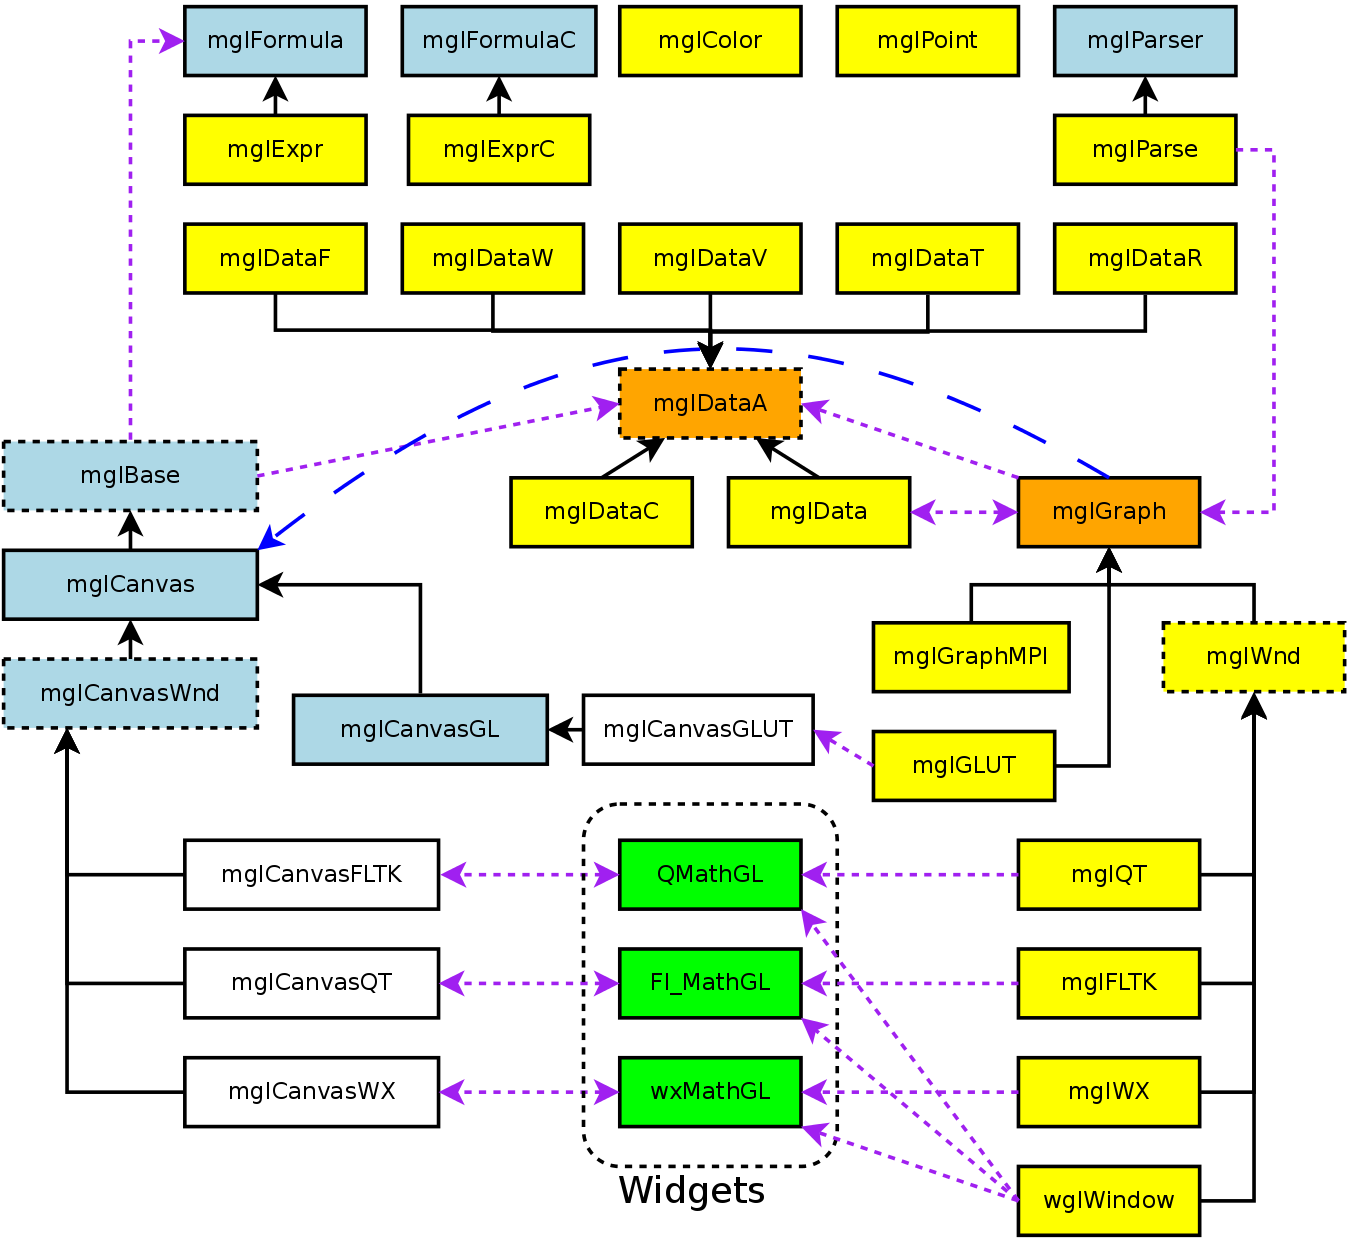
\includegraphics[width = \textwidth]{classes}
\end{frame}

\begin{frame}{Text drawing}
\includegraphics[width = \textwidth]{png/sample4-lg}
\end{frame}

\begin{frame}{Axis features}
\begin{columns}
\column{0.5\textwidth}
Curvilinear coordinates.\\
\includegraphics[width = \textwidth]{png/sample3-lg}

Log-Log scaled axes\\
\includegraphics[width = \textwidth]{png/loglog-lg}

\column{0.5\textwidth}
Several axes for one plot\\
\includegraphics[width = \textwidth]{png/2_axis-lg}

Legend for plot\\
\includegraphics[width = \textwidth]{png/legend-lg}

\end{columns}
\end{frame}

\begin{frame}{Export capabilities}
\begin{itemize}
\item Export as bitmap in PNG, JPEG or TIFF format
\item Export as vector picture EPS or SVG
\item Draws in internal GLUT or FLTK window
\item Draws in external window library as bitmap
\end{itemize}
\begin{columns}
\column{0.5\textwidth}
\includegraphics[width = \textwidth]{png/surf-lg}

\column{0.5\textwidth}
\includegraphics[width = \textwidth]{png/surf_eps.png}
\end{columns}
\end{frame}


\begin{frame}{Plot positions}
\begin{columns}
\column{0.5\textwidth}
\includegraphics[width = \textwidth]{png/sample1-lg}\\
\includegraphics[width = \textwidth]{png/ternary-lg}

\column{0.5\textwidth}
\includegraphics[width = \textwidth]{png/column-lg}\\
\includegraphics[width = \textwidth]{png/stick-lg}

\end{columns}
\end{frame}

\begin{frame}{Stereo image}
\includegraphics[width = \textwidth]{png/stereo-lg}
\end{frame}


\begin{frame}{Coloring}
\begin{columns}
\column{0.5\textwidth}
Colors are identified by single characters. In color schemes you can use brighted colors (i.e. color Id with number). MathGL use following default colors.\\
\includegraphics[width = \textwidth]{png/colors-lg}

\column{0.5\textwidth}
Color schemes are strings of color Ids. Symbol '|' disable color smoothing.\\
\includegraphics[width = \textwidth]{png/color_schemes-lg}
\end{columns}
\end{frame}

\begin{frame}{Line styles}
\begin{columns}
\column{0.5\textwidth}
Line styles and marks are also identified by characters.\\
\includegraphics[width = \textwidth]{png/sample5-lg}

\column{0.5\textwidth}
Arrows at curve edges. First symbol define arrow at the end. Second one -- at the start.\\
\includegraphics[width = \textwidth]{png/sampled-lg}
\end{columns}
\end{frame}

\begin{frame}{MGL scripts}
\begin{itemize}
\item Textual strings as commands
\item Wide spectrum of graphics and data handling commands
\item Simple structure of the language
\item Export to bitmap (PNG, JPEG, GIF) and vector (EPS, SVG) files
\item No compilation
\item WYSWYG and command line tools
\end{itemize}

\begin{columns}\small
\column{0.5\textwidth}
\texttt{\flushleft
plot dat; xrange 0 1\\
box: axis\\
xlabel 'x': ylabel 'y'\\
\# Use cycle for lines\\
for \$0 -1 1 0.1\\
line 0 0 -1 \$0 'r'\\
next}

\column{0.5\textwidth}
\includegraphics[width = \textwidth]{png/parser-lg}
\end{columns}
\end{frame}

\begin{frame}{UDAV}
\includegraphics[width = \textwidth]{main.png}
\end{frame}

\begin{frame}{Graphics in FLTK/Qt window}
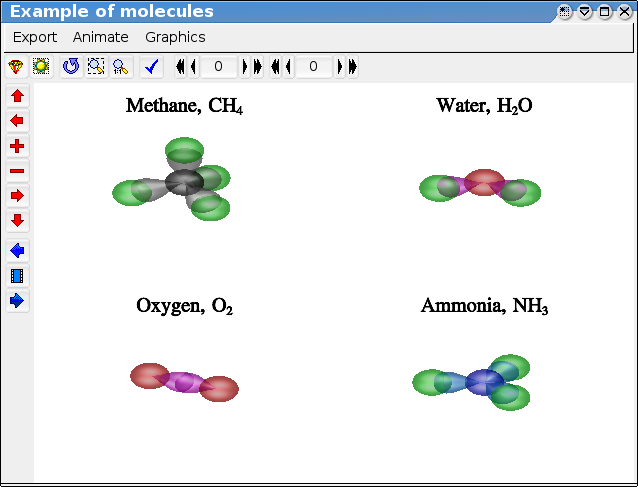
\includegraphics[width = 0.9 \textwidth]{fltk.png}
\end{frame}


\section{1D data}

\begin{frame}{Plot, Step, Tube}
\begin{columns}
\column{0.5\textwidth}
\includegraphics[width = \textwidth]{png/plot-lg}\\
\includegraphics[width = \textwidth]{png/step-lg}

\column{0.5\textwidth}
\includegraphics[width = \textwidth]{png/tube-lg}\\
\includegraphics[width = \textwidth]{png/tube_3d-lg}

\end{columns}
\end{frame}

\begin{frame}{Area, Stem, Region}
\begin{columns}
\column{0.5\textwidth}
\includegraphics[width = \textwidth]{png/area-lg}\\
\includegraphics[width = \textwidth]{png/area_2-lg}

\column{0.5\textwidth}
\includegraphics[width = \textwidth]{png/stem-lg}\\
\includegraphics[width = \textwidth]{png/region-lg}

\end{columns}
\end{frame}

\begin{frame}{Bars}
\begin{columns}
\column{0.5\textwidth}
\includegraphics[width = \textwidth]{png/bars-lg}\\
\includegraphics[width = \textwidth]{png/barh-lg}

\column{0.5\textwidth}
\includegraphics[width = \textwidth]{png/bars_2-lg}\\
\includegraphics[width = \textwidth]{png/bars_a-lg}

\end{columns}
\end{frame}

\begin{frame}{Error, Mark, BoxPlot}
\begin{columns}
\column{0.5\textwidth}
\includegraphics[width = \textwidth]{png/error-lg}\\
\includegraphics[width = \textwidth]{png/boxplot-lg}

\column{0.5\textwidth}
\includegraphics[width = \textwidth]{png/mark-lg}\\
\includegraphics[width = \textwidth]{png/textmark-lg}

\end{columns}
\end{frame}

\begin{frame}{Chart, Torus}
\begin{columns}
\column{0.5\textwidth}
\includegraphics[width = \textwidth]{png/chart-lg}\\
\includegraphics[width = \textwidth]{png/pie_chart-lg}

\column{0.5\textwidth}
\includegraphics[width = \textwidth]{png/ring_chart-lg}\\
\includegraphics[width = \textwidth]{png/torus-lg}

\end{columns}
\end{frame}


\section{2D data}

\begin{frame}{Surf}
\begin{columns}
\column{0.5\textwidth}
\includegraphics[width = \textwidth]{png/surf-lg}\\
\includegraphics[width = \textwidth]{png/surf_alpha-lg}

\column{0.5\textwidth}
\includegraphics[width = \textwidth]{png/surf_cont_fog-lg}\\
\includegraphics[width = \textwidth]{png/surf_cont_y-lg}

\end{columns}
\end{frame}

\begin{frame}{Dens, Cont, Mesh}
\begin{columns}
\column{0.5\textwidth}
\includegraphics[width = \textwidth]{png/dens-lg}\\
\includegraphics[width = \textwidth]{png/contt-lg}

\column{0.5\textwidth}
\includegraphics[width = \textwidth]{png/cont-lg}\\
\includegraphics[width = \textwidth]{png/mesh-lg}

\end{columns}
\end{frame}

\begin{frame}{Boxs, Tile, ContF, Belt}
\begin{columns}
\column{0.5\textwidth}
\includegraphics[width = \textwidth]{png/boxs-lg}\\
\includegraphics[width = \textwidth]{png/tile-lg}

\column{0.5\textwidth}
\includegraphics[width = \textwidth]{png/contf-lg}\\
\includegraphics[width = \textwidth]{png/belt-lg}

\end{columns}
\end{frame}

\begin{frame}{SurfC, SurfA, TileS, Axial}
\begin{columns}
\column{0.5\textwidth}
\includegraphics[width = \textwidth]{png/surfc-lg}\\
\includegraphics[width = \textwidth]{png/surfa-lg}

\column{0.5\textwidth}
\includegraphics[width = \textwidth]{png/tiles-lg}\\
\includegraphics[width = \textwidth]{png/axial-lg}

\end{columns}
\end{frame}


\section{3D data}

\begin{frame}{Surf3}
\begin{columns}
\column{0.5\textwidth}
\includegraphics[width = \textwidth]{png/surf3-lg}\\
\includegraphics[width = \textwidth]{png/dens_xyz-lg}

\column{0.5\textwidth}
\includegraphics[width = \textwidth]{png/cutminmax-lg}\\
\includegraphics[width = \textwidth]{png/cutminmax2-lg}

\end{columns}
\end{frame}

\begin{frame}{Cloud, Dens3, Cont3, ContF3}
\begin{columns}
\column{0.5\textwidth}
\includegraphics[width = \textwidth]{png/cloud-lg}\\
\includegraphics[width = \textwidth]{png/densa-lg}

\column{0.5\textwidth}
\includegraphics[width = \textwidth]{png/conta-lg}\\
\includegraphics[width = \textwidth]{png/contfa-lg}

\end{columns}
\end{frame}

\begin{frame}{Surf3C, Surf3A, Dots, Crust}
\begin{columns}
\column{0.5\textwidth}
\includegraphics[width = \textwidth]{png/surf3c-lg}\\
\includegraphics[width = \textwidth]{png/surf3a-lg}

\column{0.5\textwidth}
\includegraphics[width = \textwidth]{png/dots-lg}\\
\includegraphics[width = \textwidth]{png/crust-lg}

\end{columns}
\end{frame}


\section{Vector fields}

\begin{frame}{Vect, Traj}
\begin{columns}
\column{0.5\textwidth}
\includegraphics[width = \textwidth]{png/vect-lg}\\
\includegraphics[width = \textwidth]{png/vectc3-lg}

\column{0.5\textwidth}
\includegraphics[width = \textwidth]{png/vectc-lg}\\
\includegraphics[width = \textwidth]{png/traj-lg}

\end{columns}
\end{frame}

\begin{frame}{Flow, Pipe}
\begin{columns}
\column{0.5\textwidth}
\includegraphics[width = \textwidth]{png/flow-lg}\\
\includegraphics[width = \textwidth]{png/flow3-lg}

\column{0.5\textwidth}
\includegraphics[width = \textwidth]{png/pipe-lg}\\
\includegraphics[width = \textwidth]{png/pipe3-lg}

\end{columns}
\end{frame}


\section{Data handling}
\begin{frame}{Data handling (mglData)}
\Large
\begin{itemize}
\item Data may have up to 3 dimensions: $a_{ijk}$
\item Safe memory allocation, deallocation
\item Load to / save from textual files, including zipped
\item Read/write HDF4 and HDF5 files
\item Initialize uniformly or by textual formula
\item Data smoothing, differentiating, integrating, ...
\item Finding the maximum, minimum, momenta, ...
\item Getting subdatas, summation, distribution, ...
\item and so on.
\end{itemize}
\end{frame}

\begin{frame}{Fitting, Envelop, Sewing, ...}
\begin{columns}
\column{0.5\textwidth}
\includegraphics[width = \textwidth]{png/fit-lg}\\
\includegraphics[width = \textwidth]{png/envelop-lg}

\column{0.5\textwidth}
\includegraphics[width = \textwidth]{png/sew-lg}\\
\includegraphics[width = \textwidth]{png/sample6-lg}

\end{columns}
\end{frame}

\begin{frame}{PDE, Smoothing, STFA}
\begin{columns}
\column{0.5\textwidth}
\includegraphics[width = \textwidth]{png/pde-lg}\\
\includegraphics[width = \textwidth]{png/qo2d-lg}

\column{0.5\textwidth}
\includegraphics[width = \textwidth]{png/sample7-lg}\\
\includegraphics[width = \textwidth]{png/stfa-lg}

\end{columns}
\end{frame}

\section{Conclusion}
\begin{frame}{Conclusion}
\LARGE
Visit MathGL homepage\\[18pt]

http://mathgl.sf.net/\\[18pt]

for more details and download
\end{frame}
\end{document}
